\chapter{Hypothetischer Patentantrag\label{cha:chapter5}}

\section{Konfiguration für den hypothetischen Patentantrag}

Bei diesem hypothetischen Patentantrag ist das Ziel mit möglichst
wenig menschlicher Eingabe ein Patent zu erstellen,
welches durch KI entwickelt wurde.
Als KI dient hier die frei zugängliche KI ChatGPT in der Version
ChatGPT-4o benutzt im September 2024.
ChatGPT ist ein sprachgenerierendes Modell und trifft aufgrund von
Input Vorhersagen und generiert Texte nach Wahrscheinlichkeiten mit
zusätzlichen Technologien.
Es werden anders als bei RNNs alle Wörter des Outputs
gleichzeitig generiert, was eines der Grundkonzepte von 
der Technologie derTransformer
Modelle ist. Durch Self-Attention werden Beziehungen dem Modell 
Zusammenhänge zwischen Wörtern gezeigt und die menchlischeSprache antrainiert.
Die Eingabe erfolgt in natürlicher Sprache und die Ausgabe
ist ein Patentantrag, welcher die Anforderungen des Deutschen
Patent- und Markenamtes (DPMA) erfüllen soll.
Auch hier ist wichtig festzuhalten, dass eine Eingabe zwingend notwendig ist,
damit das Transformer Modell Vorhersagen für die Wörter des
Outputs treffen kann. 
Die für den Patentantrag nötigen Dokumente, welche
von ChatGPT-4o erstellt wurden, befinden sich im Appendix.
Als Branche wird hier die IOT-Branche verwendet, 
da diese ein großes Potential für die Anwendung von KI bietet.
Die Prüfung des Patentantrages findet im Gutachtenstil statt.
Für die Erteilung des hypothetischen Patentantrages offensichtliche
Punkte, werden ohne vorheriger Nennung des Gesetzestexts begutachtet.
\section{Vorbereitung der Patentanmeldung}

Um ein Patent beim DPMA anzumelden wird ein Anmeldeformular benötigt (Formular P 2790),
welches im Internet unter \url{https://www.dpma.de/docs/formulare/patent/p2007.pdf} heruntergeladen
werden kann. 
Eine ausschließlich Windows-kompatible Alternative bietet
das DPMA direktPro-System zur Online Anmeldung von Patenten.

Das Anmeldeformular verlangt:

\begin{enumerate}
    \item Angaben zum Anmelder
    \item Erfindernennung (falls abweichend vom Anmelder)
    \item Titel der Erfindung, Art der Erfindung
    \item Prioritätsangaben (falls in mehreren Ländern eingereicht)
    \item Angaben zu den Unterlagen (beigefügte Dokumente)
    \item Wahl des Prüfungsverfahrens (inhaltliche Prüfung des Antrags)
	\item Zahlungsweise
\end{enumerate}

Dabei ist zu beachten, das die Wahl des Prüfungsverfahrens 
(Rechercheantrag (§ 43 Patentgesetz)) oder
Prüfungsantrag (§ 44 Patentgesetz) zusätzliche einmalige Kosten verursacht.
Bei Auslassen der Wahl des Prüfungsverfahrens wird eine rein formulare
Prüfung des Patentantrages durchgeführt und keine inhaltliche.
Erfolgt lediglich eine Formalprüfung wird das Patent nicht erteilt.
Weitere Bestandteile der Patentanmeldung sind laut DPMA \footcite{DPMAAnmeldung}:

\begin{enumerate}
	\item Technische Beschreibung der Erfindung, gegebenenfalls mit Bezugszeichenliste
	\item Patentansprüche
	\item Zeichnungen, falls von Ihnen als notwendig erachtet
	\item Zusammenfassung
	\item Erfinderbenennung
\end{enumerate}

Diese Dokumente werden mit dem Punkt Angaben 
zu den Unterlagen (beigefügte Dokumente) abgedeckt.

\section{Erstellung KI-Patent}

Um eine durch KI entwickelte Erfindung zu generieren, 
welche möglichst wenig durch den Input beeinflusst wird, 
folgt als erster Input:
"Erstelle eine patentierbare technische Erfindung 
in Form eines Computerprogrammes im Bereich Iot" 
in ChatGPT-4o eingegeben.
Alle Inputs sind unter dem folgenden Link:
"https://chatgpt.com/share/670cf36a-b0cc-8007-aebc-73726e908c64"
einsehbar.
Die daraus entstandene Erfindung lautet:
Intelligentes Energiemanagementsystem für \gls{IoT}-basierte Haushalte.

Als Anmelder und Erfinder tritt 
wie in Kapitel 3 durch den BGH für die formelle 
Patentfähigkeit festgelegt der Benutzer
der KI in Erscheinung \ref{cha:chapter3} \ref{fig:Pat1-3}.
\begin{figure}[htb]
    \centering
    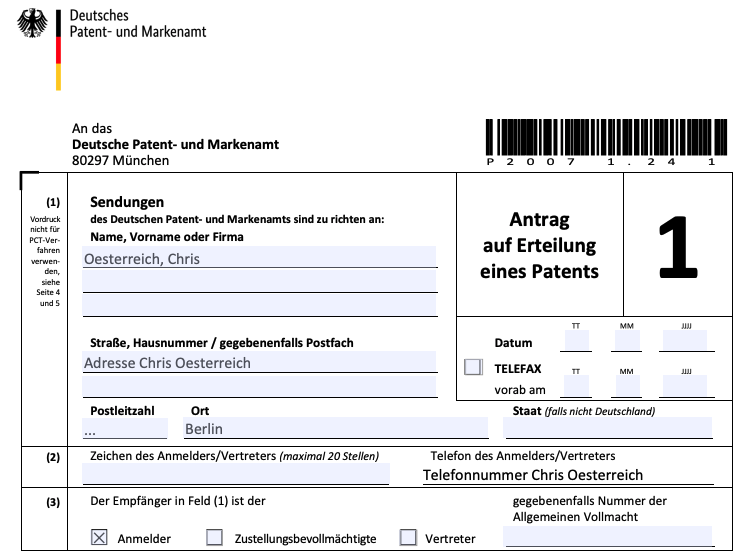
\includegraphics[width=\textwidth]{Patentanmeldung1-3.png}\\
    \caption{ Patentanmeldung Schritte 1-3 }\label{fig:Pat1-3}
\end{figure}
\\
Damit sind die Punkte "Angaben zum Anmelder" und "Erfindernennung" bearbeitet, 
da der Erfinder hier gleich dem Anmelder ist.
Die Bezeichnung der Erfindung ist:
Intelligentes Energiemanagementsystem für IoT-basierte Haushalte.
Die hypothetische Patentanmeldung enthält sowohl einen Prüfungsantrag, 
als auch einen Rechercheantrag damit die Patentanmeldung
geprüft und zum Stand der Technik auf dem Gebiet 
der Erfindung recherchiert wird um die Ähnlichkeit
zu anderen Patenten auszuschließen\ref{fig:Pat6-7}.
\begin{figure}[htb]
    \centering
    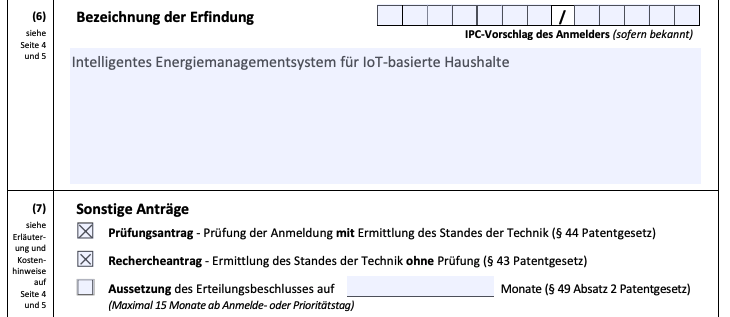
\includegraphics[width=\textwidth]{Patentanmeldung6-7.png}\\
    \caption{ Patentanmeldung Schritte 6-7 }\label{fig:Pat6-7}
\end{figure}
\\
\\
Für den Rechercheantrag fällt eine Gebühr von 300 Euro an (Stand 2024).
Für den Prüfungsantrag 150 Euro, nach vorherig gestelltem Rechercheantrag (Stand 2024).
Bei Anmeldung in Papierform bis zu 10 Patentansprüche fällt außerdem noch eine
Anmeldegebühr von 60 Euro an (Stand 2024). Bei jedem weiteren Anspruch
fallen 30 Euro pro Anspruch an(Stand 2024) Dies ergibt für das obige Patent 
eine Anmeldegebühr von 570 Euro \footcite{DPMAPatente} \ref{fig:Pat10}.
\begin{figure}[htb]
    \centering
    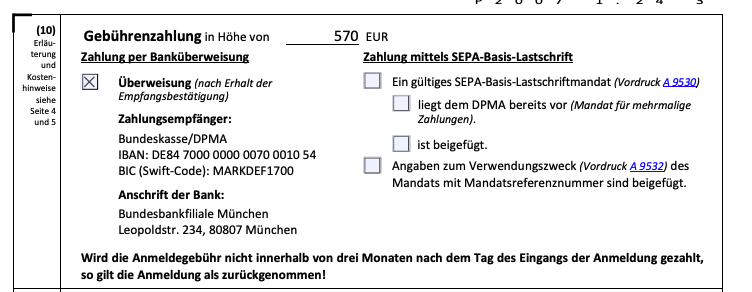
\includegraphics[width=\textwidth]{Patentanmeldung10.png}\\
    \caption{ Patentanmeldung Schritte 10 }\label{fig:Pat10}
\end{figure}

Für die oben geforderten Anlagen sind mehr Informationen von der KI
bezüglich des Patents nötig.
Als Input wird der Prompt:
"Erstelle mir die Beschreibung der Erfindung für den Patentantrag" benutzt.
Als Beschreibung der Erfindung \ref{beschPDF} gibt ChatGPT-4o eine Einordnung 
in das technische Gebiet, den Stand der Technik, die Problemlösung,
die technischen Merkmale , sowie Vorteile der Erfindung zurück.
Nach der Erstellung der Beschreibung werden durch einen weiteren Input:
"Erstelle mir die Schutzansprüche für die Anmeldung des oben genannten Patents?"
die detaillierten Patentansprüche \ref{schutzPDF} 
zurückgegeben.
Eine Zusammenfassung \ref{zusammenfassungPDF} muss ebenfalls
generiert werden über die Eingabe:
"Erstelle mir eine Zusammenfassung der Erfindung". 
Damit wären die Grundbestandteile der Patentanmeldung erfüllt und nach Angabe der 
Zahlungsweise und
Einreichung der Anmeldung beim DPMA würde die Prüfung beginnen. 

\section{Die durch KI erschaffenen technischen Computerprogramme}
Die durch ChatGPT-4o und die Eingabe entstandene Erfindung nutzt Machinelles Lernen um eine effiziente
Energieverwaltung in Haushalten zu ermöglichen. 
Dafür werden Daten gesammelt und mithilfe von maschinellen Lernen Muster 
und Vorhersagen getroffen um Geräte in den Standby zu schalten 
oder vor erwarteter Benutzung aufzuwecken. 
Die zu patentierenden Computerprogramme wären bei dieser Erfindung die
Patentansprüche 1,3,4,8 (2.Hauptanspruch),9,10 aus \ref{schutzPDF}. 
Der erste Schutzanspruch ist einer von zwei Hauptansprüchen 
und beschriebt ein System zur Optimierung des Energieverbrauchs in IoT-basierten SmartHomes.
Das Computerprogramm, welches mittels Machine Learning
auf den Kompenenten des SmartHomes das technische Problem
der Energiesteuerung löst könnte patentierbar sein.
Ebenso könnten einzelne Bestandteile davon ebenfalls patentierbar sein,
wie die Unteransprüche drei und vier.
Unteranspruch drei bezieht sich auf den Machine-Learning Algorithmus,
welcher anhand historischer Daten Verhaltensmuster erkennt \ref{lst:schutz3}. 
Unteranspruch vier ist ein prädiktiver Steuerungsalgorithmus ,
welcher basierend auf den Vorhersagen 
den Betriebsstatus der IoT-Geräte steuert \ref{lst:schutz4}.
Der zweite Hauptanspruch beschreibt ein Verfahren zum Erfassen von Daten, 
Analysieren mittels Machine-Learning-Algorithmen 
und Vorhersagen des zukünftigen Energieverbrauchs. 
Während der erste Hauptanspruch ein System zur
Energiesteuerung beschreibt, welches aus 
Soft und Hardwarekomponenten besteht, 
beschreibt der zweite Hauptanspruch ein Verfahren zur Optimierung 
mithilfe des Systems. Auch dieses Verfahren wird durch ein 
Computerprogramm realisiert und löst das technische Problem 
der Energiesteuerung in IoT-basierten SmartHomes.
Zu diesem Hauptanspruch gehören zwei Unteransprüche mit Bezug auf 
Computerprogramme, der Unteranspruch neun und Unteranspruch zehn.
Der Unteranspruch neun beschreibt die Analyse der gesammelten
Daten anhand von historischen Datene, dem Energiepreis 
und anderen äußeren Faktoren, wie den Wetterbedingungen mittels
eines Computerprogrammes \ref{lst:schutz9}. 
Unteranspruch zehn hingegen befasst sich mit der Optimierung 
des Energieverbrauchs durch den vorrausschauenden 
Einsatz von Energiesparmodi und Standby-Zuständen \ref{lst:schutz10}.

\paragraph{Recherche zum Stand der Technik}
Im Bereich von Intelligentes Energiemanagementsystem sind beim DPMA die Patente
10 2016 223 981.3, 10 2020 126 756.8 und 60 2022 005 048.0 gelistet. Das Patent
10 2016 223 981.3 (System und Verfahren für intelligentes Energiemanagementsystem im Fahrzeug)
von der Bayerische Motoren Werke Aktiengesellschaft wertet Kartendaten aus 
und schaltet anhand dieser Sensoren bzw. Berechnungsmodule ab oder an.
Die angemeldeten Schutzansprüche \footcite{DPMAregisterRecherchierbarerText} beziehen
sich alle auf Technologien innerhalb eines Fahrzeuges.
Das Patent 10 2020 126 756.8 (INTELLIGENTES ENERGIEMANAGEMENTSYSTEM FÜR EIN FAHRZEUG UND ENTSPRECHENDES VERFAHREN)
\footcite{DPMAregisterRecherchierbarerTexta} enthält ebenfalls nur
Patentansprüche mit Bezug auf Fahrzeuge.
Das Patent 60 2022 005 048.0 (INTELLIGENTES ENERGIEMANAGEMENTSYSTEM (IEMS) UND GLEICHGEWICHTSPROFIL)
\footcite{DPMAregisterRecherchierbarerTextb} bezieht sich auf ein System zur Steuerung eines Schiffs
mit Fokus auf die Effizienz und Redundanz der Geräte. 
Trotz der unterschiedlichen technische Anwendungsbereiche gibt 
es im Detail Gemeinsamkeiten zwischen der zu prüfenden Patentanmeldung 
und dem Patent 60 2022 005 048.0. 
Beide Systeme beinhalten eine Benutzeroberfläche und
nutzen Machine-Learning-Algorithmen. 
Während das Schiffssystem Machine Learning(ML) benutzt um Berechnungen 
der Effizienz- und Redundanzwerte vorzunehmen, verwendet das Smart Home
System ML zur Erkennung von Verhaltensmustern 
und zur Vorhersage des Energieverbrauchs. Die Benutzeroberfläche
des Schiffssystems zeigt die besten Geräteeinstellungen auf,
im Gegensatz zum Smart Home System, wo die 
Benutzeroberfläche eine Schnittstelle für die
Überwachung und Optimierung des Energieverbrauchs bietet.
Es ist hier genauer zu überprüfen, inwiefern die 
angewandten Methoden sich unterscheiden und ob sie Ähnlichkeit aufweisen.
Der Hauptanspruch 1 des Schiffssteuerungssystems, könnte
mit den Ansprüchen 1,4,8 des Smart Home Systems in Konflikt stehen.
Ebenso Unteranspruch 3,4 des Schiffssteuerungssystems mit Unteranspruch 3 des Smart Home Systems,
sowie Unteranspruch 6 des Schiffssteuerungssystems mit Unteranspruch 9 des Smart Home Systems.
Die Recherchen unter der Eingabe "intelligente IOT" ergibt keine relevanten Treffer.
Die Eingabe "IOT Energie" liefert das Patent 60 2016 088 465.8 
(VERFAHREN ZUR ENERGIE- UND LEISTUNGSVERWALTUNG FÜR INTERNET DER DINGE (IOT) UND SCHALTMETHODE),
welches potenziell ähnliche Methoden benutzt wie das Smart Home System.
Jedoch bezieht sich dieses Patent auf ein batteriebetriebenes Gerät
und eine Hardwarelösung,
welche den Energieverbrauch durch spannungsbasierte Schaltungen und Transistoren reduziert.

\section{Prüfung der Schutzansprüche}
Die Prüfungsstelle des Deutschen Patent- und Markenamts (DPMA) könnte die Erteilung eines
Patents gemäß § 49 Abs. 1 PatG beschließen.
\subsection{Formelle Vorrausetzungen}
Die formellen Voraussetzungen müssten gegeben sein.
\subsubsection{Anmeldung}
Die Erfindung müsste zur Erteilung eines Patents beim Patentamt angemeldet worden sein (§ 34 Abs.
1 PatG).
\\
Dabei wird angenommen,
das die Anmeldung in Papierform erfolgt und die Anmeldegebühr bezahlt ist. 
Somit liegt eine Anmeldung vor.
\subsubsection{Form}
Gemäß § 34 Abs. 3 PatG muss die Anmeldung den Namen der/des Anmelders*in (Nr. 1), einen
Antrag auf Erteilung des Patents, in dem die Erfindung kurz und genau bezeichnet ist (Nr. 2), einen
oder mehrere Patentansprüche (Nr. 3), eine Beschreibung der Erfindung (Nr. 4) sowie die
Zeichnungen, auf die sich die Patentansprüche oder die Beschreibung beziehen (Nr. 5), enthalten.
\\
Als Erfinder tritt bei diesem Patentantrag der Nutzer der
KI auf, da dieser als Einziger eine Eingabe getätigt hat und
laut Beschluss des BGH als Erfinder auftreten kann ohne die Wahrheitspflicht
zu verletzen \footcite{BPatG21122021}. 
Der Name des Anmelders ist hier gleich dem Erfinder und bei der
Anmeldung angegeben. 
Die Erfindung ist kurz und genau bezeichnet und die Patentansprüche, 
eine Beschreibung der Erfindung
sind vorhanden. 
Kein Patentanspruch oder die Beschreibung bezieht sich auf Zeichnungen
und somit sind keine vorhanden.
\\
Die Erfindung ist deutlich und vollständig offenbart, 
so dass eine Fachfrau
oder ein Fachmann sie ausführen kann (§ 34 Abs. 4 PatG) und die
Anmeldung enthält nur eine einzige zusammenhängende Erfindung(§ 34 Abs. 5 PatG). 
\\
Die Erfindungsbeschreibung genügt, dass ein Fachmann das System, sowie 
das Verfahren nachbauen kann, insbesondere durch die Angabe des Codes
ist es möglich mit wenig Anpassungen das System(Hauptanspruch 1) oder
das Verfahren(Hauptanspruch 2) nachzubauen.Das der Code noch auf die speziellen
Geräte angepasst werden muss, steht der deutlichen und vollständigen
Offenbarung nicht entgegen. Es wird ein grundlegendes
Verständnis von Machine Learning und Energiemanagement vorausgesetzt,
welches ein Fachmann im Bereich IOT besitzt. Die Erfindung ist klar und
und vollständig definiert.
\\
Somit genügt die Anmeldung den Anforderungen der §§ 34, 37 und 38 PatG.
\subsubsection{Gerügte Mängel}
Gerügte Mängel liegen keine vor (§ 45 Abs. 1 PatG)
\subsection{Materielle Vorrausetzungen}
Der Gegenstand der Anmeldung müsste nach §§ 1 – 5 PatG patentfähig sein. (§ 49 Abs. 1 PatG)

\subsubsection{Technizität}
Bei dem Gegenstand der Anmeldung müsste es sich um eine Erfindung auf einem Gebiet der Technik
handeln (§ 1 Abs. 1 PatG).
In Kapitel \ref{sec:tecer} befindet sich eine Definition des Gebietes 
der Technik, welche sich nach Haedicke zwar nicht abschließend definieren
lässt, jedoch genug Einblick gewährt um die Schutzansprüche zu bewerten.
Da es laut Urteil vom 30.6.2015 \footcite{BGH3020152015} ausreicht wenn 
eine "... beanspruchte Lehre den Einsatz technischer Geräte umfasst", ist
die Frage der Technizität bei Patentanmeldungen von Verfahren und 
Systemen im Zusammenhang mit IOT hinreichend geklärt.
Der Begriff IOT beschreibt technische Geräte, welche miteinander 
kommunizieren und somit sind die Schutzansprüche auf einem Gebiet der Technik
angesiedelt.
Art. 1 Abs. 3 PatG legt Gegenstände und Tätigkeiten fest, die nicht als Erfindung i.S.v. § 1 Abs. 1 PatG
angesehen werden. Diese Gegenstände oder Tätigkeiten als solche sind nicht patentfähig (§ 1 Abs. 4
PatG). So werden laut Gesetzestext insbesondere
Entdeckungen sowie wissenschaftliche Theorien und mathematische Methoden (§ 1 Abs. 3 Nr. 1
PatG),
ästhetische Formschöpfungen (§ 1 Abs. 3 Nr. 2 PatG),
Pläne, Regeln und Verfahren für gedankliche Tätigkeiten, für Spiele oder für geschäftliche Tätigkeiten
sowie Programme für Datenverarbeitungsanlagen (§ 1 Abs. 3 Nr. 3 PatG) sowie
die Wiedergabe von Informationen (§ 1 Abs. 3 Nr. 4 PatG),
nicht als Erfindungen i.S.v. § 1 Abs. 1 PatG angesehen.
[§ 1 Abs. 2 PatG, § 1a PatG u. § 2a PatG]
Bei Computerprogrammen ist es wichtig, dass 
"verfahrensbestimmende Anweisungen enthalten (sind), welche die Lösung eines konkreten
technischen Problems mit technischen Mitteln zum Gegenstand haben“ \footcite{BGH2020092009}.
Die Schutzansprüche 1,3,4,8,9,10 beziehen sich auf die Lösung eines technischen Problems
mit technischen Mitteln. Das Computerprogramm regelt dabei die Umsetzung der 
Lösung des Problems des Energiemanagement mithilfe von technischen Geräten.
Der Gegenstand der Anmeldung stellt somit eine Erfindung auf einem Gebiet der Technik dar.



\subsubsection{Neuheit}
Die Erfindung müsste neu sein (§ 1 Abs. 1 i.V.m. § 3 PatG).
Eine Erfindung gilt als neu, wenn sie nicht zum Stand der Technik gehört (§ 3 Abs. 1 S. 1 PatG). Der
Stand der Technik umfasst alle Kenntnisse, die vor dem für den Zeitrang der Anmeldung
maßgeblichen Tag durch schriftliche oder mündliche Beschreibung, durch Benutzung oder in
sonstiger Weise der Öffentlichkeit zugänglich gemacht worden sind (§ 3 Abs. 1 S. 2 PatG).
Als Stand der Technik gilt auch der Inhalt nationaler Patentanmeldungen in der beim Deutschen
Patentamt ursprünglich eingereichten Fassung mit älterem Zeitrang, die erst an oder nach dem für
den Zeitrang der jüngeren Anmeldung maßgeblichen Tag der Öffentlichkeit zugänglich gemacht
worden sind (§ 3 Abs. 2 Nr. 1 PatG) […] [Stoffe und Stoffgemische, § 3 Abs. 3, 4 PatG).
Für die Anwendung von § 3 Abs. 1 und Abs. 2 PatG bleibt eine Offenbarung der Erfindung außer
Betracht, wenn sie nicht früher als sechs Monate vor Einreichung der Anmeldung erfolgt ist und
unmittelbar oder mittelbar zurückgeht auf einen offensichtlichen Missbrauch zum Nachteil des
Anmelders oder seines Rechtsvorgängers (§ 3 Abs. 5 Nr. 1 PatG). […]

Entgegen der Neuheit des Patentanspruches steht die Patentanmeldung 60 2022 005 048.0.
Nach Prüfung der angewandten Methoden unterscheiden diese sich jedoch deutlich und eine Ähnlichkeit
ist nicht gegeben. Obwohl die Benutzung von Machine Learning und Energiemanagement
in dem Bereich IOT nicht neu ist, wurden noch keine Patente dafür ausgestellt.
Jedoch ist die Erfindung in ähnlicher Form schon stand der Technik.
In einem Paper von \footcite{energymanagement} wird ein System    
beschrieben, welches Machine Learning Algorithmen benutzt um den Energieverbrauch
in Haushalten zu optimieren. Zudem wird auf Literatur verwiesen, 
welche sich ebenfalls eingehend mit dem Thema befasst.
Die Erfindung ist nicht neu. 

Der Patentantrag wird hilfsgutachterlich weiter geprüft.




\subsubsection{Erfinderische Tätigkeit}
Die Erfindung müsste auf einer erfinderischen Tätigkeit beruhen (§ 1 Abs. 1 i.V.m. § 4 PatG).
Eine Erfindung gilt als auf einer erfinderischen Tätigkeit beruhend, wenn sie sich für den Fachmann
nicht in naheliegender Weise aus dem Stand der Technik ergibt (§ 4 S. 1 PatG). Gehören zum Stand
der Technik auch Unterlagen im Sinne des § 3 Abs. 2 PatG, so werden diese bei der Beurteilung der
erfinderischen Tätigkeit nicht in Betracht gezogen (§ 4 S. 2 PatG).
\\
Der Output der KI könnte als Erzeugnispatent patentierbar sein,
falls dieser für einen Fachmann nichtnaheliegend ist.
Da der Einsatz einer KI, wenn sie in der Branche üblich ist keine besondere
Erfindungshöhe aufweist, ist zu prüfen, inwieweit KI in der IOT Branche
als Standardwerkzeug gilt und wie hoch bei dieser Erfindung der menschliche 
Anteil ist. Im Bereich der Entwicklung neuer IOT-Systeme ist es Standard auf
die Hilfe von KI zurückzugreifen. 
Ein Fachmann, der sich mit IoT-Technologien befasst, wird daher mit der Anwendung von KI 
vertraut sein. 
Dies umfasst den Einsatz von KI-Algorithmen für Datenanalyse, 
Automatisierung, Echtzeit-Verarbeitung und Mustererkennung.
Die KI hat die Erfindung in Form eines Computerprogrammes erstellt,
welches die Energieverwaltung in Haushalten optimiert.
Die Erfindung basiert auf Machine Learning Algorithmen, welche
historische Daten analysieren und Verhaltensmuster erkennen.
Die Verwendung von historischen Verhaltensmustern und prädiktiven
Analysen ist bereits ein bekannter Ansatz im Bereich IOT.
Es
ist naheliegend Machine-Learning zu verwenden, 
sowie aus historischen Daten prädiktive Analysen
zu erstellen um 
Energieverbräuche zu optimieren. Ein
Beispiel für ein ähnliches System ist 
Google Nest \footcite{YourHelpfulHome}.
Das von Google entwickelte "Nest Learning Thermostat" verwendet
ebenfalls ML, lernt aus dem Verhalten der Nutzer und
optimiert den Energieverbrauch.
Die KI-Erfindung ist herstellerunabhängig, während
die meisten herstellergebunden sind. Trotzdem ist 
diese Idee nicht neu und es gibt schon 
offene Smart-Home-Plattformen und Standards.

In den Schutzansprüchen 1,3,4,8 (2.Hauptanspruch),9,10
befinden sich keine für den Fachmann nicht naheliegenden
Systeme oder Verfahren. Auch der Code gibt keinen
Hinweis auf eine erfinderische Tätigkeit.

Jedoch wäre ein Verfahrenspatent, welches hier nicht als Schutzanspruch vormuliert
ist theoretisch patentierbar, in dem die Verwendung von LLMs zur 
Erstellung von Patentanträgen als neuartig und erfinderisch angesehen wird.
ChatGPT und ähnliche Modelle gehören zur Kategorie der Large Language Models (LLMs), 
die darauf trainiert sind, menschliche Sprache zu verstehen und zu generieren. 
In der IoT-Branche wird KI üblicherweise für Aufgaben wie Datenanalyse, 
Mustererkennung, Anomalieerkennung und Automatisierung eingesetzt. 
Die Verwendung eines sprachbasierten KI-Modells 
in der IoT-Branche ist weniger verbreitet, jedoch
in spezifischen Fällen, wie der Sprachsteuerung, vorzufinden.
Vorallem die Verwendung von ChatGPT als kreatives Werkzeug 
zur Erfindung technischer Lösungen im Kontext des Patentrechts, 
ist noch kein etablierter Ansatz. Für einen im Patentrecht definierten Fachmann, 
der mit klassischen Methoden der Forschung und Entwicklung vertraut ist, 
wäre die Idee, ein Sprachmodell wie ChatGPT zur 
Konzeption eines technischen Systems einzusetzen, nicht unmittelbar naheliegend.
Der menschliche und kreative Anteil ist dann auf die Idee zu 
kommen ein LLM zu diesem Zweck zu nutzen.
Dies könnte als erfinderische Tätigkeit angesehen werden,
wurde hier jedoch nicht als Schutzanspruch gestellt.

Mithin beruht die Erfindung auf keiner erfinderischen Tätigkeit.
\subsubsection{Gewerbliche Anwendbarkeit}
Die Erfindung müsste gewerblich anwendbar sein (§ 1 Abs. 1 i.V.m. § 5 PatG).
Eine Erfindung gilt als gewerblich anwendbar, wenn ihr Gegenstand auf irgendeinem gewerblichen
Gebiet einschließlich der Landwirtschaft hergestellt oder benutzt werden kann (§ 5 PatG).
Ein System zur intelligenten Steurung von Geräten in einem IOT-Haushalt ist gewerblich anwendbar,
genauso wie Verfahren, welche dieses System unterstützen.
Die Erfindung ist gewerblich anwendbar.


\subsubsection{Ausschluss}
Die Patentierbarkeit ist nicht ausgeschlossen.

\subsection{Gesamtergebnis}
Die Prüfungsstelle des Deutschen Patent- und Markenamts (DPMA) wird die Erteilung eines
Patents gemäß § 49 Abs. 1 PatG nicht beschließen.